\chapter{Visualizing Scene Graphs}


\section{Desiderata}
Before we're able to implement our possible scene graph models, 
Visualizing the richly structured geometric information contained in a generative scene graph model is vital for proper debugging and analysis of modeling and inference programs.
The most basic requirement is visualizing the components of our scene graph representation $(G, \Theta, Z)$.
It is important to be able to clearly distinguish each part of our representation;
as we see later, incorrect behavior in any part of our model or inference can introduce huge variation in the posterior and inferred approximation.
Observed neural detections can be visualized as a special-case scene graph with no edges.
As such, this covers a point-estimate view of the majority of addresses in the scene graph models we explored.

On top of this, we'd also like to capture some information about distributions over scene graphs.
Providing an clearly interpretable view of all possible distributions $p(G, \Theta, Z)$ is a huge task, so we restrict ourselves to sample-based approximations of unimodal distributions over continuous parameters, and relatively small numbers of structures.
Within this class of scenes, common characterizing features are the mean and uncertainty, so our visualizations should provide a clear view of one or more of these features.


\section{Examples}
\subsection{Visualizing a Single Scene Graph}
\begin{figure}[t]
  \centering
  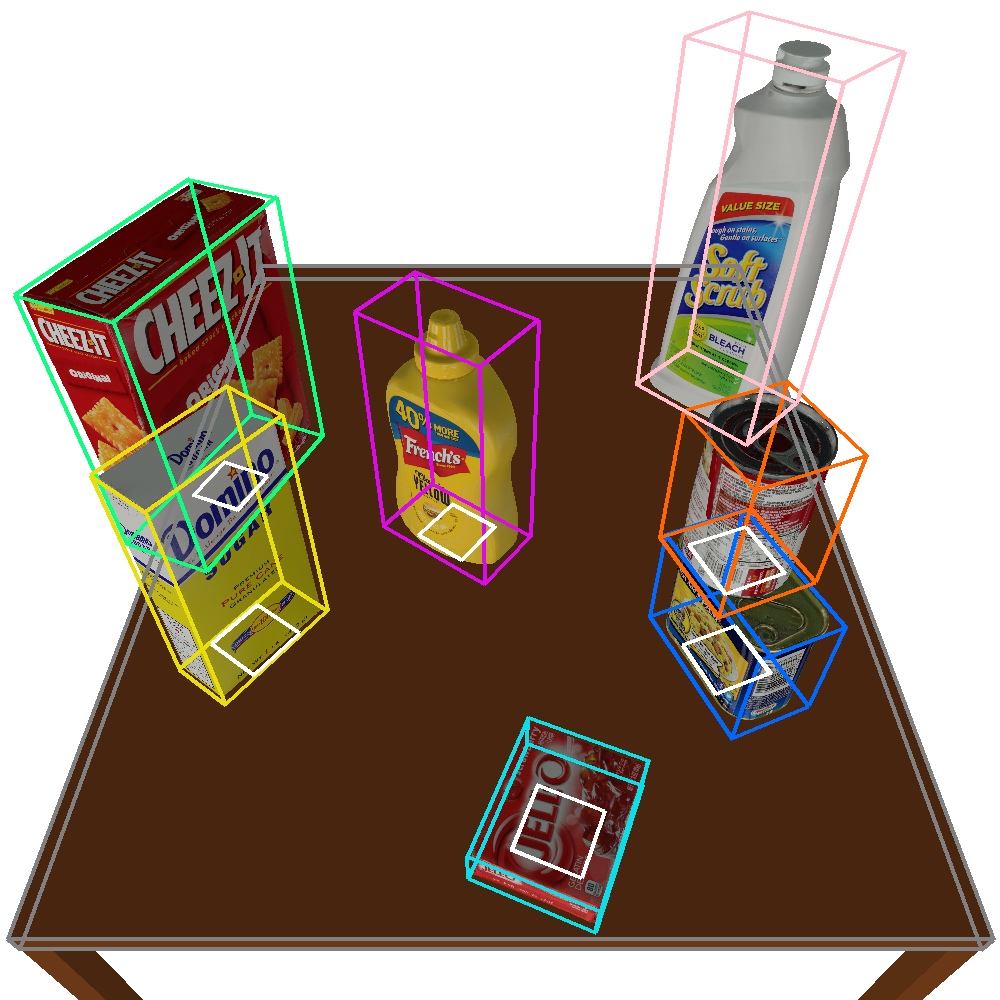
\includegraphics[scale=0.35]{overlaidSceneGraph}
  \caption{
    Visualization of a synthetic scene with its abstract scene graph overlaid.
  }
  \label{fig:overlaidSceneGraph}
\end{figure}

Our main utility is a function that accepts an image, a scene graph $(G, \Theta, Z)$ where $G = (V,E)$, and a camera configuration, and renders that scene graph as a wireframe representation overlaid on top of the image, as viewed from the provided camera specification.
Figure~\ref{fig:overlaidSceneGraphs} demonstrates using this function to see a synthetic rendered scene's underlying scene graph.
For each object $o \in O$ in the scene graph, the function renders a colored wireframe bounding box with the dimensions of $o$, and 6DoF pose given by $x_o$.
Importantly, this is the \textit{absolute} pose of the object, including any slack in relative contacts.
Thus, the continuous parameters $\Theta := \{\theta_e\}_{e \in E}$ are not explicitly used in rendering, but can be distinguished in contacting objects $i,j \in O$ by the distance in their corresponding wireframe renderings.
Contact edges $e \in E$ are visualized as white squares, located at the center of face $f_i$.
Face $f_j$ is not directly visualized, but can often be inferred from which face is closest to $f_i$.
This does not preclude potential ambiguity for certain pathological slack terms that rotate $i$ close to a multiple of $\pi/2$.
However, in practical modeling applications we find such occurrences to be rare, as sensible priors weight heavily against large slack terms.

\subsection{Distributions over Structure Beliefs}
\begin{figure}[t]
  \centering
  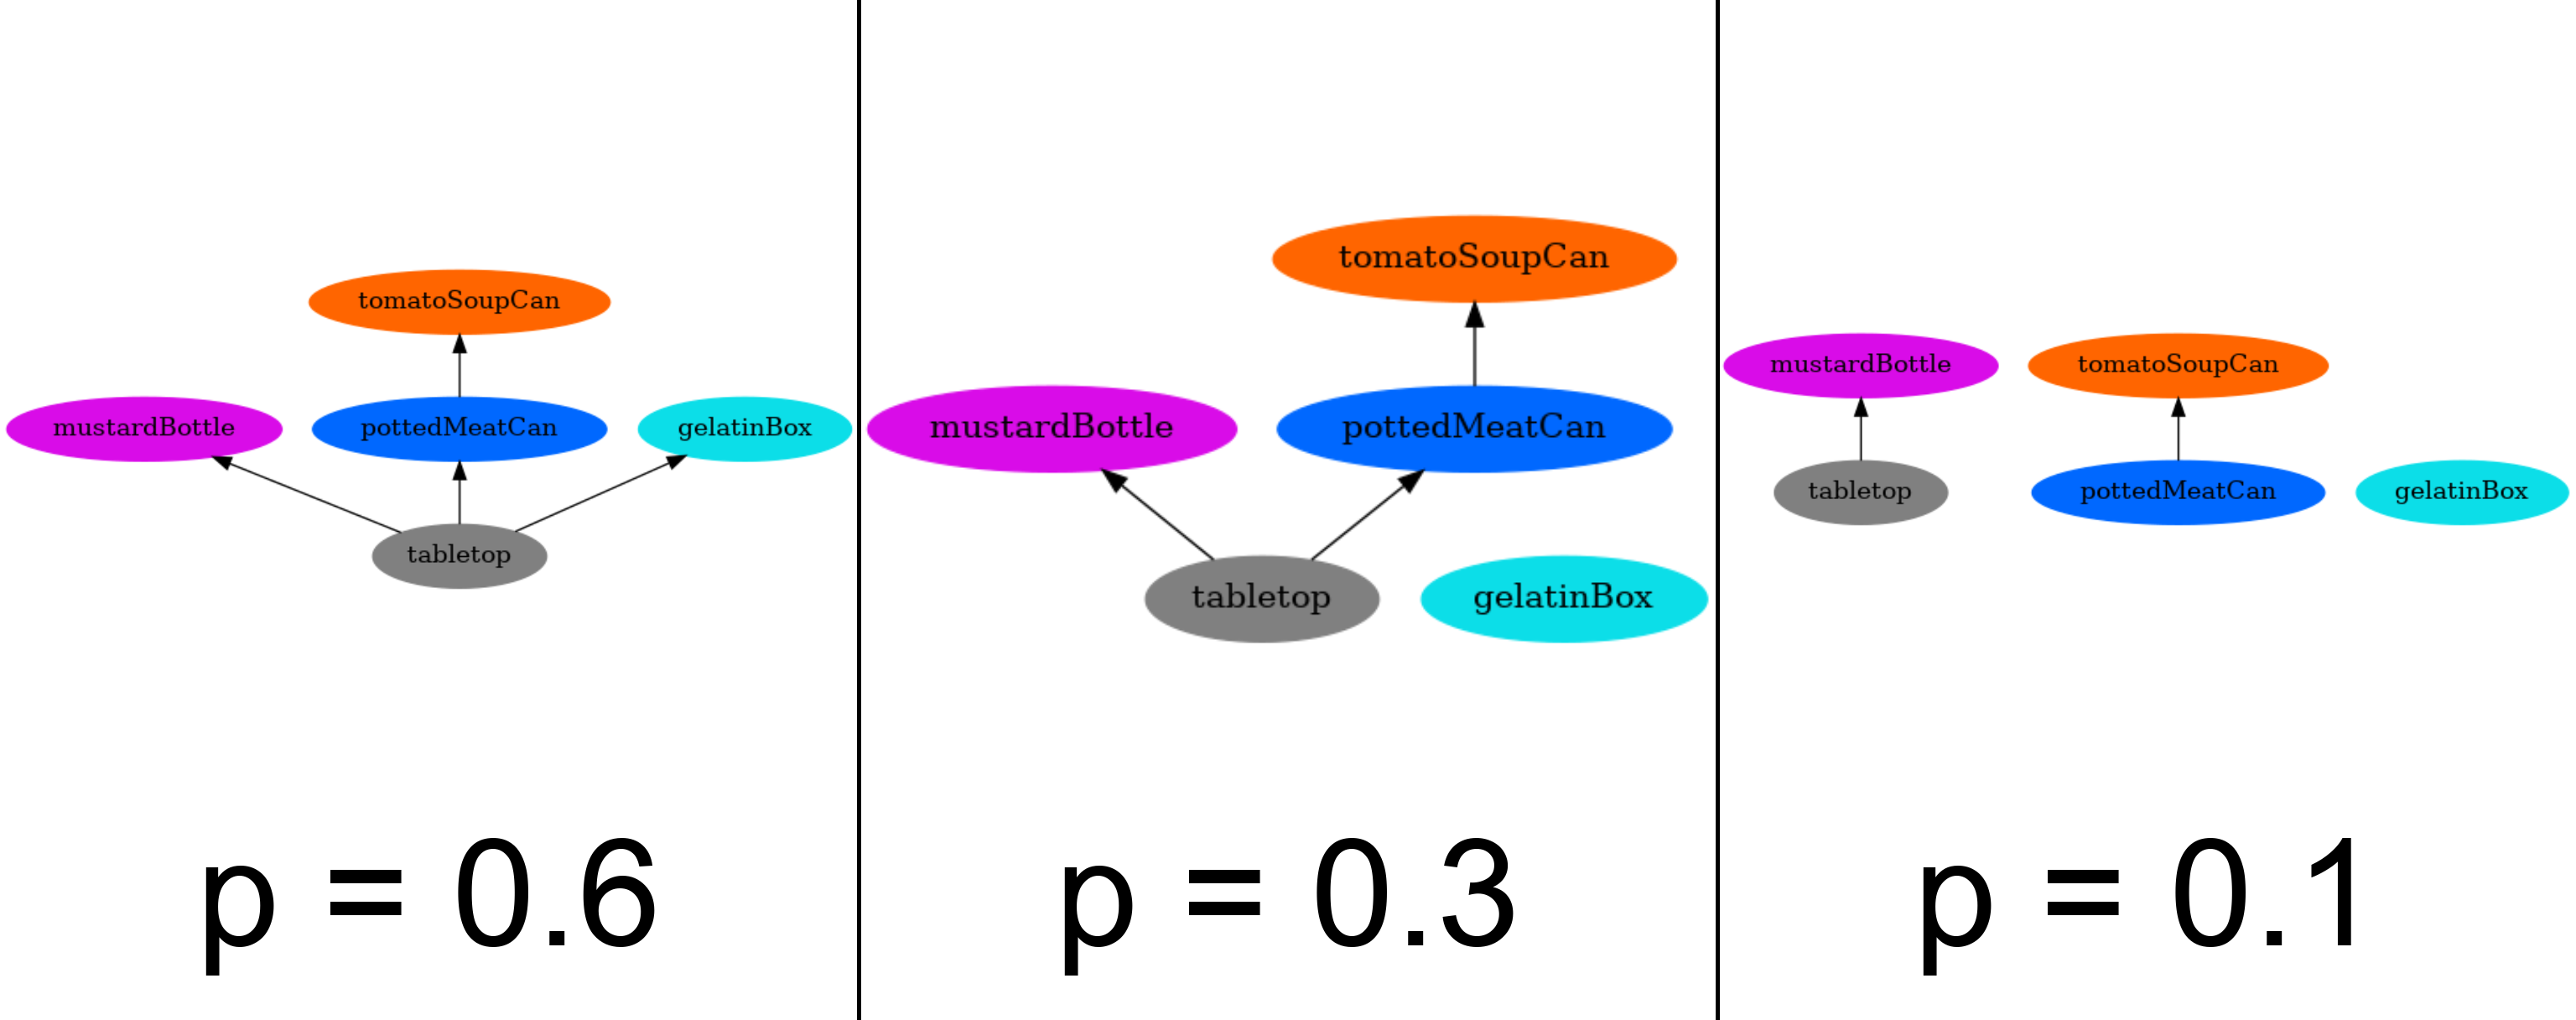
\includegraphics[scale=0.125]{structureDistribution}
  \caption{
    Visualization of a distribution over abstract scene graph structure using Graphviz.
  }
  \label{fig:structureDistribution}
\end{figure}

As we will quickly see, using the utility shown in Figure~\ref{fig:overlaidSceneGraph} quickly runs into issues displaying multiple structures over the same image.
Since edges are rendered roughly in the same place, it can be hard to tell exactly how many samples have an edge between any two given objects.
Even more, it's virtually impossible to tell which vertices and edges are part of the same scene graph.
We develop a utility based off the Graphviz~\cite{Ellson03graphvizand} graph visualization library to more clearly view different discrete structures.
It accepts a distribution over scene graphs, and renders a specified number of the most probable present in a scene.
In Figure~\ref{fig:structureDistribution}, we can see how this clearly represents the top competing hypotheses for scene graph structure.
This tool can be combined with the wireframe overlay to give rich visualizations of distributions over scene graphs.

\subsection{Distributions over Scene Beliefs}
\begin{figure}[H]
  \begin{subfigure}[b]{\textwidth}
    \centering
    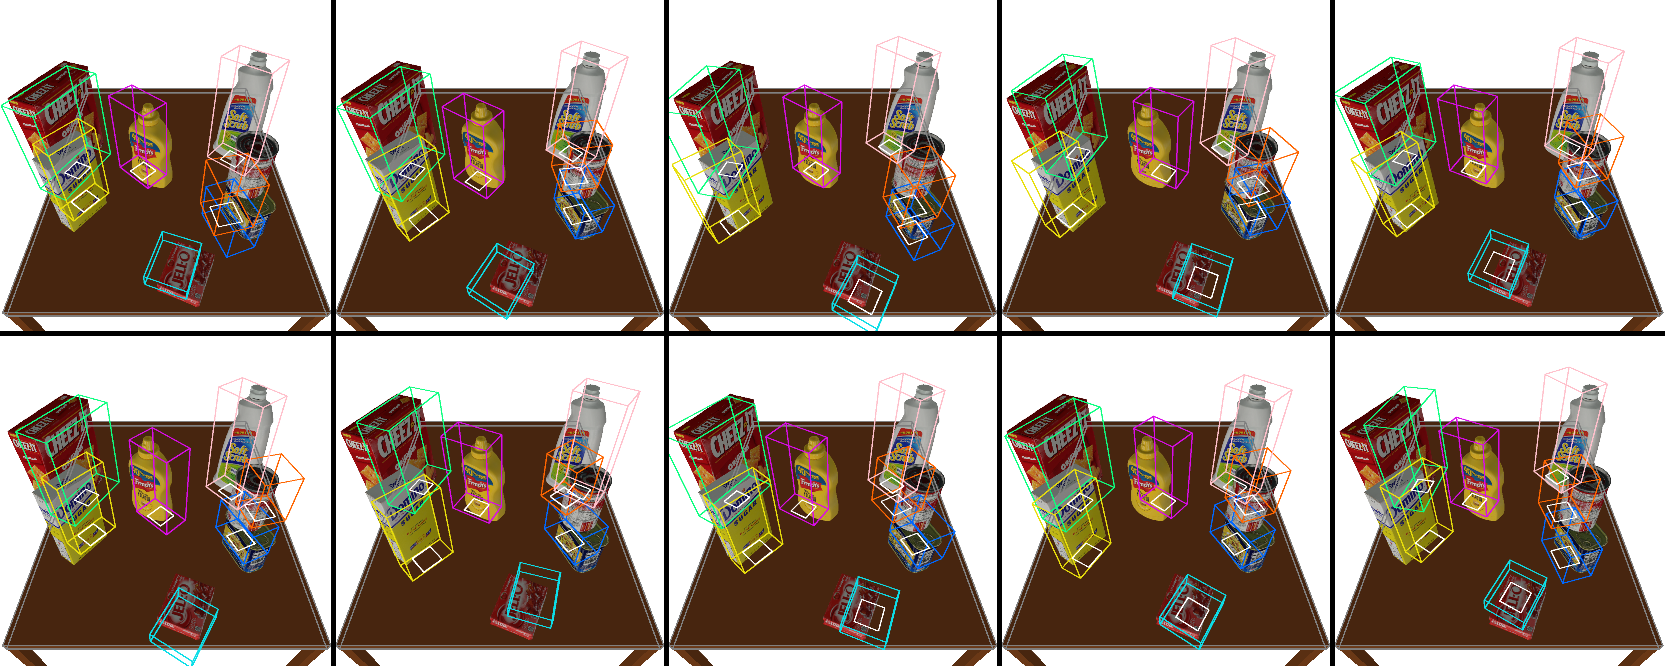
\includegraphics[scale=0.25]{multipleBeliefsTop}
    \caption{
      Visualization of each sample's state using our scene graph visualization utility.
    }
    \label{fig:multipleBeliefsTop}
  \end{subfigure}
  \begin{subfigure}[b]{\textwidth}
    \centering
    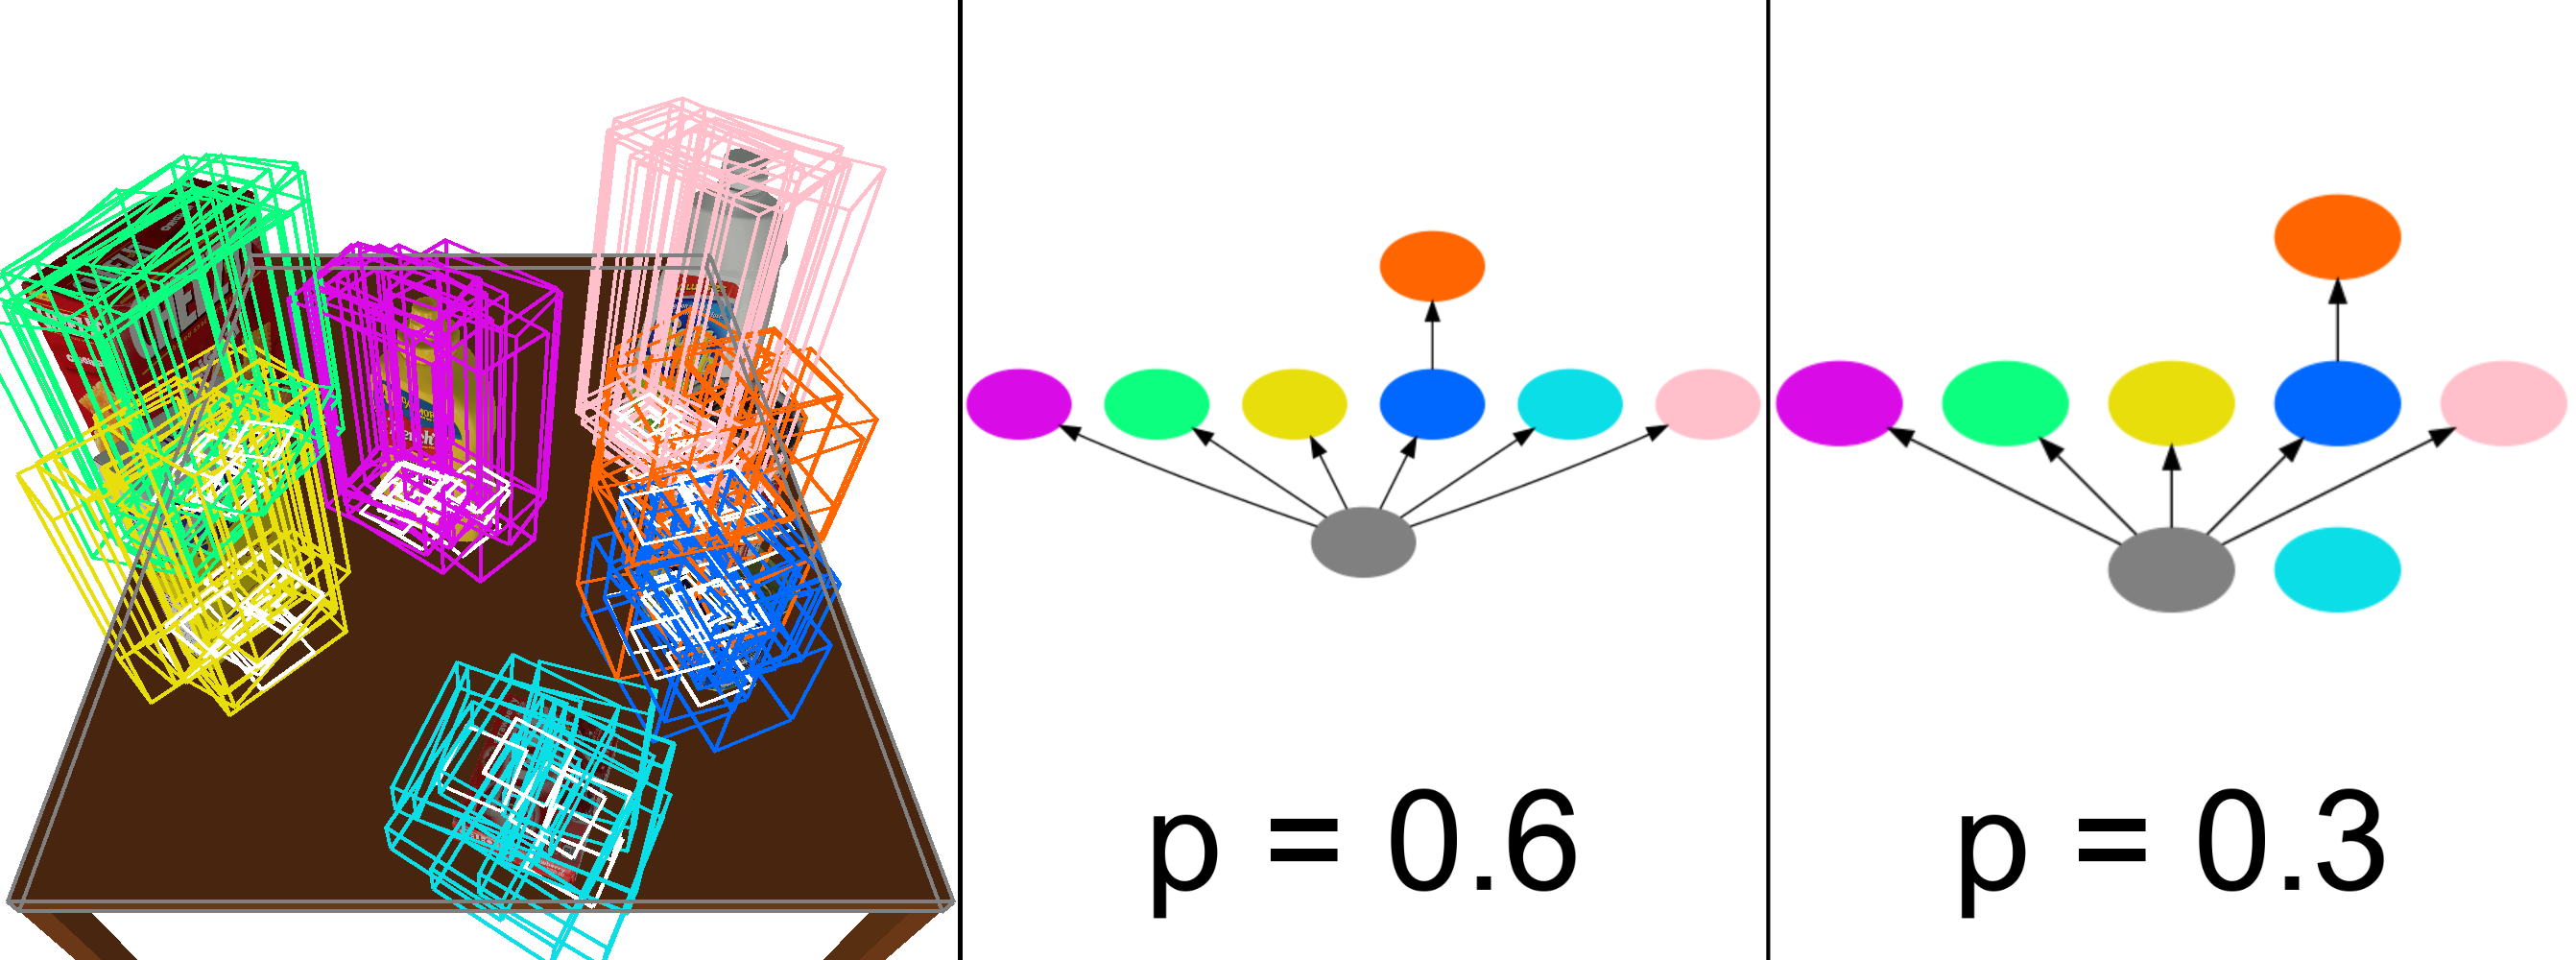
\includegraphics[scale=0.15]{multipleBeliefsMiddle}
    \caption{
      All 10 samples, rendered over the same image. Only the two most frequent structures are shown.
    }
    \label{fig:multipleBeliefsMiddle}
  \end{subfigure}
  \begin{subfigure}[b]{\textwidth}
    \centering
    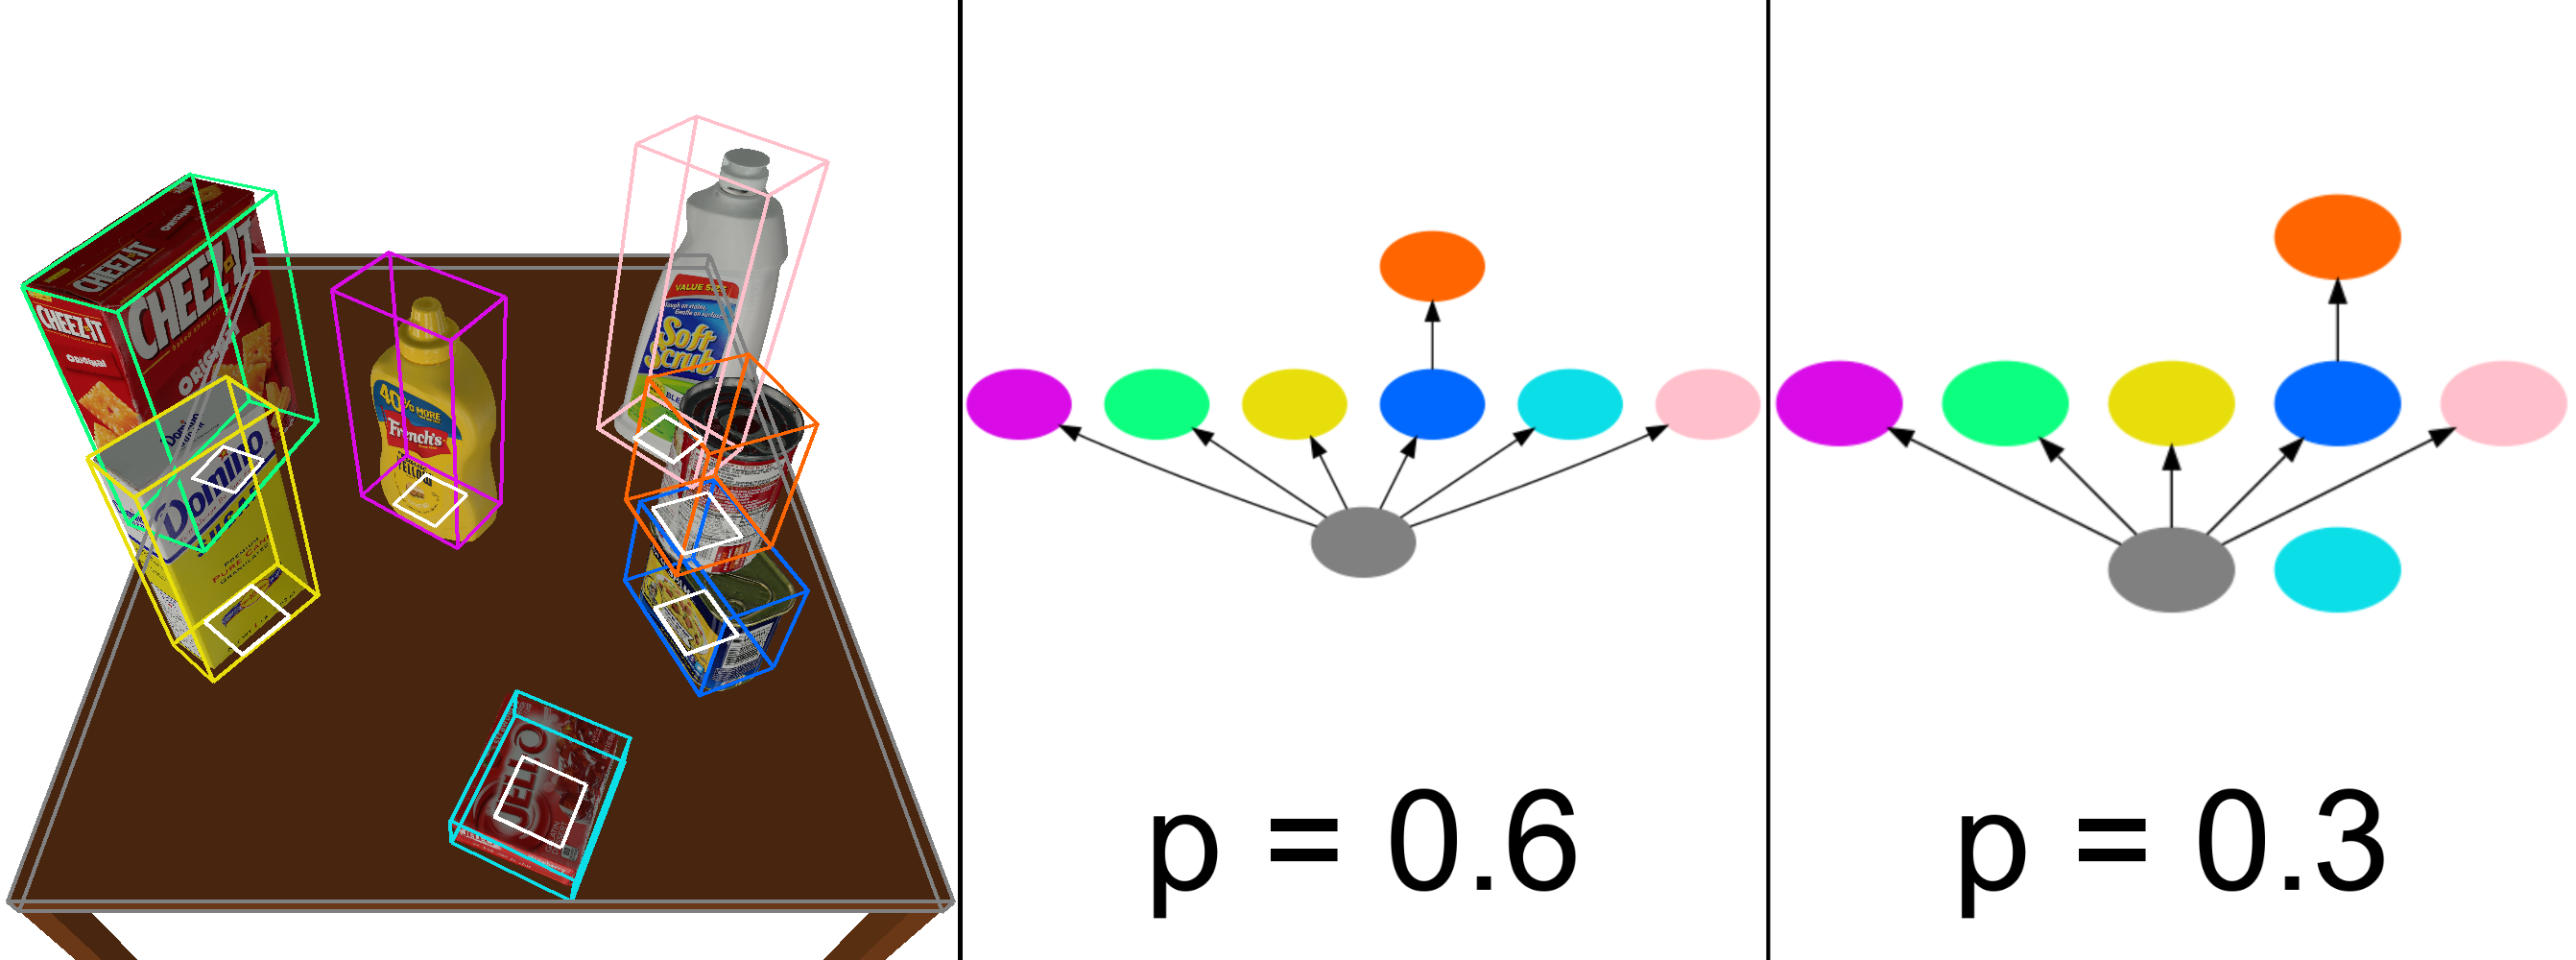
\includegraphics[scale=0.15]{multipleBeliefsBottom}
    \caption{
      Aggregated visualization of all the samples. Only the two most frequent structures are shown.
    }
    \label{fig:multipleBeliefsBottom}
  \end{subfigure}
  \caption{
    Various methods for visualizing multiple beliefs.
    Node labels are omitted in the rendered structure distribution, and instead the wireframe rendering and GraphViz node for an object $o$ share the same color.
  }
  \label{fig:multipleBeliefs}
\end{figure}

We can now combine our utilities to render rich views of multiple samples.
To generate our example visualization distribution, we generate 10 scene graphs $\{\mathcal{G}_i\}_{i \in 1:10}$, with object parameters sampled from a uniform distribution centered at the true scene graph as seen in Figure~\ref{fig:overlaidSceneGraph}.
Figure~\ref{fig:multipleBeliefsTop} shows the simplest form of visualizing the collection of samples, as a collage of separate renderings of each sample.
This provides the most information, but at a glance it's difficult to get a sense of the mean and uncertainty of the distribution its representing.

We instead try aggregating the separate samples into a single representative ``belief'' $\mathcal{G}^* = \mathrm{agg}(\{\mathcal{G}_i\}_{i \in 1:N})$ that is then overlaid on top of the rendered scene.
We can then composite this with the abstract structure visualization to improve our ability to see uncertainty in scene structure.

One possible aggregation method is simply taking the disjoint union $\mathrm{agg}(\{\mathcal{G}_i\}_{i \in 1:N}) = \displaystyle\bigsqcup_{i=1}^N \mathcal{G}_i$.
As we see in Figure~\ref{fig:multipleBeliefsMiddle}, this has the effect of overlaying all of the beliefs on top of the same image.
This can give a sense of the amount of uncertainty in object positions and rotations, but obscures the underlying object, making it difficult to determine the accuracy of the pose beliefs.

The second method we try $\mathrm{agg}(\{\mathcal{G}_i\}_{i \in 1:N}) = (G^*, \Theta^*, Z^*)$ first takes the most probable structure $G^* = \argmax_G\ \hat{p}(G, \Theta, Z)$ among our samples.
The discrete parameters $Z^*$ are then selected arbitrarily from one of the graphs that has this structure.
We then let the continuous parameters $\Theta^*$ be determined by the average of that scene's objects' absolute poses $x_o^* = \mathrm{avg}(\{x_{(i,o)}\}_{i \in 1:N})$ across all other samples (the average position uses a simple sum, while the average orientation is calculated using the method described by Markley et. al in \cite{markley2007averaging}).
Figure~\ref{fig:multipleBeliefsBottom} shows an example of this method.
In contrast to the Figure~\ref{fig:multipleBeliefsMiddle}, this method clearly shows the accuracy of pose beliefs, but loses information about uncertainty in the continuous parameters. These trade-offs mean choosing a visualization is somewhat contextually dependent on if the accuracy or uncertainty is more relevant.

\begin{figure}[H]
  \includegraphics{particleFilterVis}
  \caption{
    Visualization of sampling and rejuvenation moves in a particle filter.
    A complete video of this scene can be seen at: \url{https://www.youtube.com/watch?v=0_0TvrGC65Q}.
    (i) shows the first time step with the overlaid beliefs from the initial time step prior (initialized to the observed neural pose estimates), before structure inference.
    (ii) shows the beliefs over the first time step, after running 1 step of the rejuvenation kernel.
    (iii) shows the beliefs over the second time step, after sampling from the dynamics model.
    (iv) shows the beliefs over the second time step, after running 20 steps of the rejuvenation kernel.
  }
  \label{fig:particleFilterVis}
\end{figure}

\subsection{Visualizing Inference in a Particle Filter}
Finally, we demonstrate a real-world application by showing the actual usage of these visualization utilities in a particle filter with a corresponding complex inference program.
The scene graph model we used leverages the prior from \todo[cite prior scene graph model section] and dynamics from \todo[cite scene graph model dynamics].
Object poses are initialized to their observed neural detections in the first time step.
The inference program leverages a rejuvenation MCMC kernel after sampling from the prior for the first and second time step.
This kernel is in turn composed of an interleaved RJMCMC kernel (see \todo[cite RJMCMC section]) for discrete structure, and a drift kernel for continuous parameters.
We run the particle filter with 10 particles, and 20 iterations of the rejuvenation kernel.
Figure~\ref{fig:particleFilterVis} leverages the visualization method seen in Figure~\ref{fig:multipleBeliefsBottom} to aggregate the particle filter state into a stable visual estimate of the mean object poses, and to view the distribution over inferred structure.
This example shows how we can leverage the methods introduced in this chapter in practice for visualizing and debugging complex inference programs.
